A Tabela \ref{tab:tempos_bubble} apresenta os tempos de execução, em segundos, obtidos para o Bubble Sort nos seis tamanhos de instância exigidos pelo trabalho, para cada um dos três tipos de entrada testados.

\begin{table}[htbp]
    \centering
    \begin{tabular}{|l|r|r|r|r|r|r|}
        \hline
         & 10 & 100 & 1.000 & 10.000 & 100.000 & 1.000.000 \\
        \hline
        Crescente & 0,000001 & 0,000001 & 0,000000 & 0,000003 & 0,000033 & 0,000321 \\
        \hline
        Decrescente & 0,000002 & 0,000002 & 0,000166 & 0,015925 & 1,583171 & 155,625005 \\
        \hline
        Random & 0,000003 & 0,000008 & 0,000326 & 0,027070 & 8,899341 & 938,659248 \\
        \hline
    \end{tabular}
    \caption{Tempo de execução (em segundos) do Bubble Sort por tamanho e tipo de instância}
    \label{tab:tempos_bubble}
\end{table}


O Gráfico \ref{fig:grafico_bubble} apresenta esses mesmos dados em escala linear. Assim como no Insertion Sort, a entrada crescente permanece praticamente em zero em todos os tamanhos (graças à parada antecipada do algoritmo), enquanto as entradas decrescente e randômica crescem de forma acentuada a partir de 100.000 elementos. Diferentemente do Insertion Sort, porém, aqui a entrada randômica é a mais lenta das três: para 1.000.000 de elementos, 938,7 s, contra 155,6 s da entrada decrescente.

\begin{figure}[htbp]
    \centering
    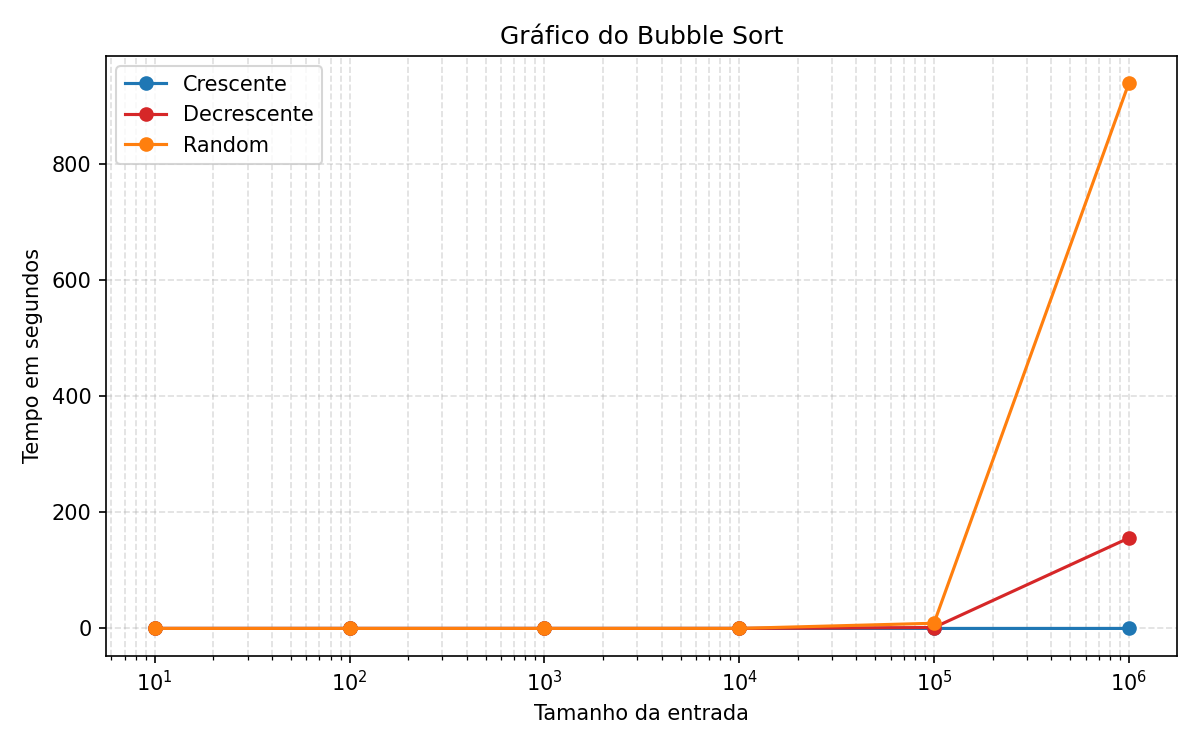
\includegraphics[width=14cm]{Imagens/Bubble Sort/grafico.png}
    \caption{Gráfico de tempo por tamanho do algoritmo Bubble Sort (escala linear)}
    \label{fig:grafico_bubble}
\end{figure}

O Gráfico \ref{fig:grafico_bubble_log} em escala logarítmica confirma o comportamento linear da entrada crescente e o comportamento quadrático das entradas decrescente e randômica. O tempo de 0,000000 s medido para 1.000 elementos na entrada crescente (abaixo da resolução do relógio, de cerca de 1 $\mu$s) não pode ser representado em escala logarítmica, e por isso a curva da entrada crescente apresenta uma interrupção nesse ponto.

\begin{figure}[htbp]
    \centering
    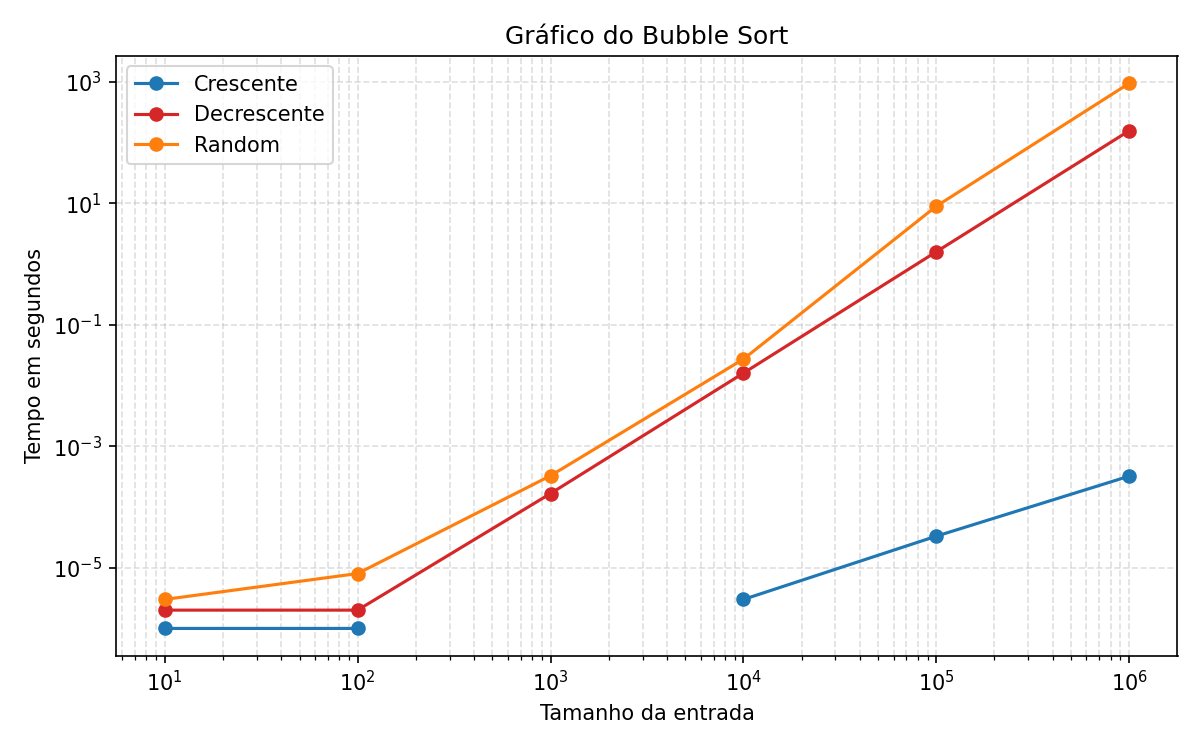
\includegraphics[width=14cm]{Imagens/Bubble Sort/grafico_log.png}
    \caption{Gráfico de tempo por tamanho do algoritmo Bubble Sort (escala logarítmica)}
    \label{fig:grafico_bubble_log}
\end{figure}

Comparando com o Insertion Sort (Capítulo 1), nota-se que, na entrada decrescente, os dois algoritmos tiveram desempenho equivalente (155,6 s para o Bubble Sort contra 167,0 s para o Insertion Sort, para 1.000.000 de elementos), enquanto na entrada randômica o Bubble Sort foi cerca de 11,6 vezes mais lento (938,7 s contra 80,6 s). Parte dessa diferença é explicada pelo número de comparações: em uma entrada aleatória o Bubble Sort realiza cerca de $n(n-1)/2$ comparações, o dobro das cerca de $n(n-1)/4$ do Insertion Sort. A diferença restante provavelmente decorre de efeitos de hardware, discutidos na análise de complexidade deste capítulo, que a simples contagem de operações não captura.
